\documentclass[a4paper,13pt]{article}
\usepackage[MeX]{polski}
\usepackage[hidelinks]{hyperref}
\usepackage{color}
\usepackage{mathtools}
\usepackage[OT4]{fontenc}
\usepackage{listings}
\usepackage[margin=1in]{geometry}
\usepackage{float}
\floatstyle{plaintop}
\restylefloat{table}

\frenchspacing




\lstset{
	language=C++,
	breaklines=true,
	postbreak=\mbox{\textcolor{red}{$\hookrightarrow$}\space},
	literate={ą}{{\,a}}1 {ę}{{\,e}}1 {ó}{{\'o}}1 {ż}{{\*z}}1 {ź}{{\'z}}1 {ł}{{\'l}}1 {ś}{{\'s}}1 {ć}{{\'c}}1 {ń}{{\'n}}1
}


\title{Projekt robota trójnożnego}
\author{Jakub Mazur}
\date{\today}


\begin{document}

%\begin{lstlisting}
%ą ę ż ł
%\end{lstlisting}
% TODO - ogarnąć encoding


\maketitle

\hypersetup{
	linktocpage=true,
    colorlinks=true,
    urlcolor=red,
    linktoc=all,
    linkcolor=blue,
}
\tableofcontents

\section{Wstęp}
\subsection{Historia robotów kroczących}
Pierwsza idea robota kroczącego pojawiła się już pod koniec XV wieku, a narodziła się w głowie nikogo innego jak Leonarda Da Vinci. Od tamtej pory wielu naukowców próbowało tworzyć konstrukcje, które używały nóg zamiast kół. Jednakże, pierwsze faktycznie udane roboty tego typu datuje się dopiero na początek lat 60 ubiegłego wieku. Pojawiły sie wtedy pierwsze działające konstrukcje, na przykład robot czteronożny zbudowany przez Josepha Shingleya oraz roboty sześcio i ośmonożne zbudowane przez "Space General Corporation". \cite{history}\\

Od tamtej pory powstało wiele różnych projektów, które kategoryzuje się w zależności od ilości nóg posiadanych przez robota:\\
\begin{itemize}
	\item jednonożne
	\item dwunożne (Humanoid, chicken-walkers)
	\item czteronożne (Quadrupedal)
	\item sześcionożne (Hexapod)
	\item ośmionożne
	\item gąsiennicowe
\end{itemize}

Można tu zaobserwować pewną tendencję spadkową, wraz z upływem czasu widać wzrost udanych konstrukcji o mniejszej ilości nóg. Konstrukcje takie wymagają większej wiedzy naukowców, lepiej dobranych algorytmów ale za to można je skonstruować mniejszym nakładem materiałowym. Stąd naturalne jest dążenie do ograniczania ilości nóg w konstrukcjach robotów kroczących\\

Pojawia się także inna tendencja w ilości nóg robotów. Prawie wszystkie konstrukcje (poza jednonożnymi) opierają się na anatomii zwierząt. Jest to raczej logiczna tendencja, jako że do takich robotów mamy już algorytmy chodu opracowane przez miliony lat ewolucji. Biologiczne "konstrukcje", które nie mają sensu nie przetrwałyby do dziś. \cite{history}\\

Co natomiast z konstrucjami robotów trójnożnych? Można się zastanowić czy konstrukcje takie nie powstają ponieważ faktycznie nie mają sensu, czy może dlatego że temat bardziej "klasycznych", prostszych w implementacji, konstrukcji nie został po prostu jeszcze wyczerpany przez naukowców. Jeżeli rozejrzymy się dookoła siebie możemy zaobserwować wiele przedmiotów codziennego użytku które posiadają właśnie trzy nogi, od wszelakich taboretów, przez wieszaki na ubrania po stoły. Są to jednak przedmioty statyczne i dla takich rozwiązań trzy nogi są wymaganym minimum aby dany przedmiot stał stabilnie. Co jednak z konstrukcjami dynamicznymi? Jeżeli robot trójnożny podniesie nogę, straci stabilność, zacznie się przewracać. Czyni to z niego dość ciekawą konstrukcję, gdzie w momencie stania w miejscu zachowuje się bardzej jak roboty o większej ilości nóg, nie przewraca się, a podczas ruchu zachowuje się jak roboty dwunożne, musi odpowiednio szybko odstawić nogę w odpowiednie miejsce aby się nie przewrócić.\\

\subsection{Istniejące konstrukcje trójnożne}
Konstrukcje trójnożne pojawiały się w dziełach science fiction już od dawna, od "The War of the Worlds" z 1898 aż po "Mroczne Widmo" z 2001 i regularnie pojawiają się naukowcy, którzy próbują udowodnić że nie trzeba ogarniczać tego typu robotów do dzieł z obszaru science fiction.\\
\subsubsection{STriDER} 
Został zbudowany w 2007 na Uniwersytecie Stanowym w Virginii. Jego celem były eksperymenty z algorytmami chodu i doclewo, prowadzenie obserwacji. Miały to umożliwić długie nogi, które znacznie podwyższały konstrukcję i sprawiały że górna platforma była idealna do instalowania wszelakiego rodzaju urządzęń typu kamery. Kinematykę robota można określić jako $3-SRRR$, a kinematykę jednej nogi jako $RRR$. Przy czym "pierwsze" $R$ oznacza obrót dookoła osi $x$ a dwa kolejne $R$ oznaczają obrót wokół osi $y$ (zgodnie z oznaczeniami na rysunku \ref{strider_math})  \cite{strider}\\

\begin{figure}[H]
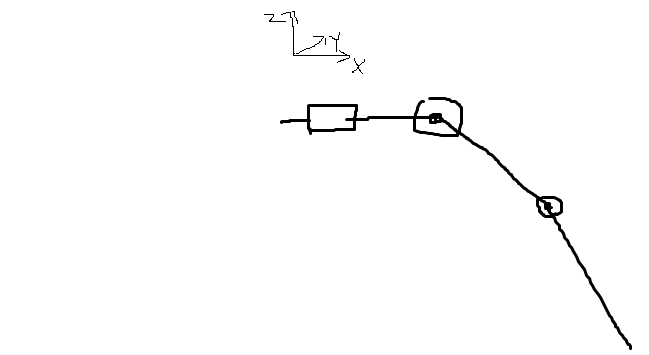
\includegraphics[width=\textwidth]{img/strider_math.png}
\caption{Uproszczony model matematyczny nogi robota STriDER}
\label{strider_math}
\end{figure}

\subsubsection{Triped "Martian" }
Jest to robot zbudowany przez Yoichi Masudę na uniwersytecie w Osace w 2017 roku. Kinematyka tego robota opiera się na mechaniźmie SLIP (Spring-Loaded-Inverted Pendulum). SLIP ma w pewien sposób symulować sposób poruszania się stosowany przez ludzi i zwierzęta. Sprężyna wewnątrz nogi robota jest naciągana, co powoduje skracanie się nogi, a zwalnianie sprężyny z powrotem wydłuża człon. Dodatkowo dodane jest serwo, które może obracać nogę dookoła osi $y$. Czyni to z nogi robota mechanizm o kinematyce typu $RL$. Został także dodany czujnik naprężenia, który jest w stanie zmierzyć siłę naciągu nici kompresującej sprężynę. \cite{Triped Martian}\\

\begin{figure}[H]
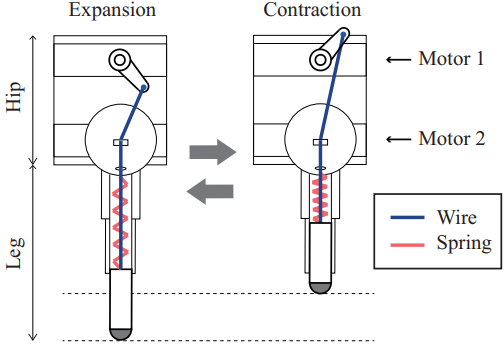
\includegraphics[width=0.5\textwidth]{img/martian_model.png}
\caption{Model nogi robota Triped Martian źródło: \cite{Triped Martian}}
\label{martian_leg}
\end{figure}

\subsubsection{Inne konstrukcje}
W internecie można także znaleźć kilka różnych, niezbyt dobrze udokumentowanych konstrukcji zakończonych mniejszym lub większym sukcesem:
\begin{itemize}
\item \href{https://makerfaire.com/maker/entry/71669/}{Makerfaire 3-legged walking robot}
\item \href{https://youtu.be/HGEhCCUgFMg}{missel tripod robot}
\end{itemize}

Niestety konstrukcje te nie posiadają żadnej dokumentacji technicznej i nie da się dokładnie określić zasady ich działania. Nie można nawet mieć pewności że konstrukcje te faktycznie istnieją a nie są oszustwem lub inną formą naginania rzeczywistości, na co mogłaby wskazywać jakość filmików i uboga ilość materiałów.\\

\section{Model Matematyczny}

\subsection{Noga robota typu RRR}

Noga ma trzy stopnie swobody. Wszystkie są typu obrotowego, co czyni z niej konstrukcję typu $RRR$. Przy czym dwa elementy rotacyjne obracają się dookoła osi poziomej ($X$) (podobnie jak w przypadku robota STriDER), a jedna dookoła osi pionowej ($Z$). Są to też te same osi obrotu co w przypadku ramienia robotycznego typu antromorficznego (zwanego także "angular" bądź "jointed"). Co za tym idzie, cały model matematyczny jest w zasadzie identyczny jak w przypadku manipulatora tego typu.\\

\begin{figure}[H]
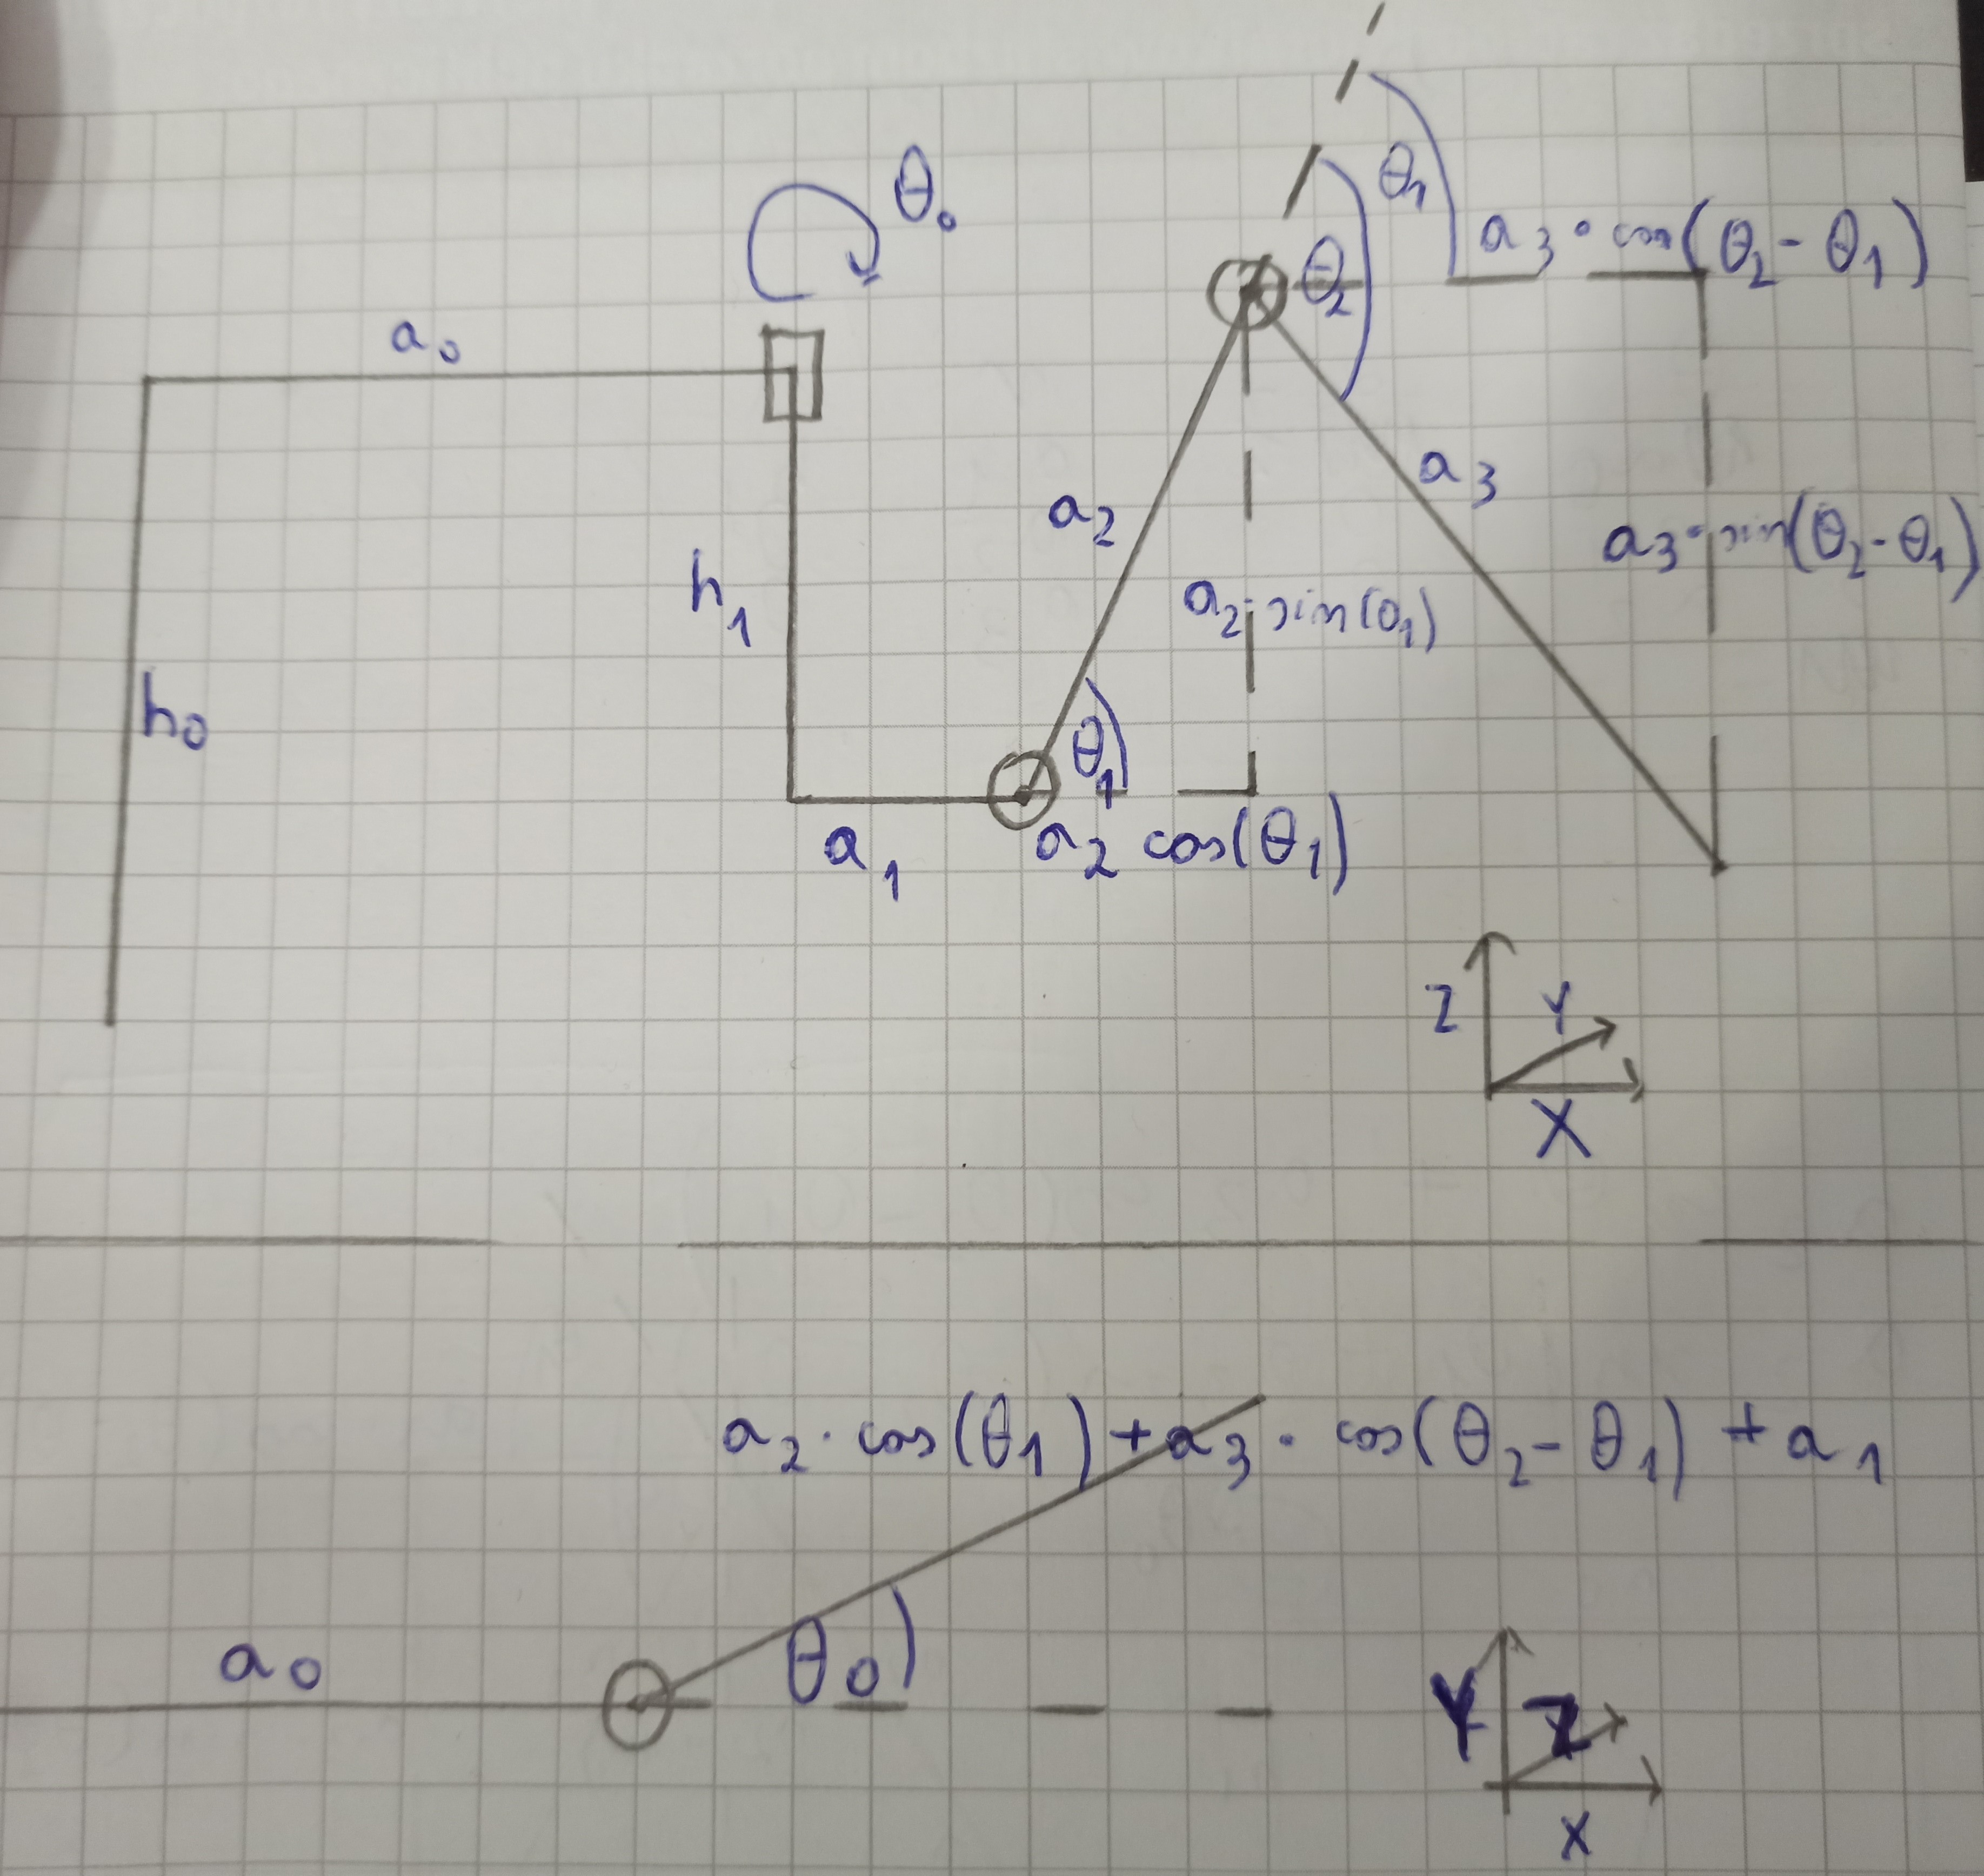
\includegraphics[width=\textwidth]{img/math_model.jpg}
\caption{Model Matematyczny}
\label{math_model}
\end{figure}

\subsubsection{Kinematyka Prosta}
Obliczanie kinematyki prostej polega na uzyskniu równań końcówki ramienia robotycznego we współrzędnych kartezjańskich względem współrzędnych konfiguracyjnych. Inaczej mówiąc, wejściem algorytmu jest zbiór współrzędnych konfiguracyjnych, a na wyjściu otrzymamy współrzędne kartezjańskie.\cite{robot_manipulators}\\

W przypadku tego konkretnego manipulatora, mamy do czynienia z trójwymiarowym układem współrzędnych kartezjańskich i trzema stopniami swobody. Da to liniowo niezależny układ trzech równań, w którym parametrami będą kąty na jakich mają ustawić się serwomechanizmy a wynikiem wektor współrzędnych kartezjańskich.\\

Najprostszą metodą liczenia kinematyki prostej jest rozrysowanie modelu matematycznego i geometryczne wyprowadzenie potrzebnych równań. Model taki dla tego manipulatora został przedstawiony na rysunku \ref{math_model}. Przyjęty początek układu współrzędnych został oznaczony jako $(0, 0, 0)$, a punkt którego współrzędne kartezjańskie są poszukiwane został oznaczony jako $(X, Y, Z)$. $h_1$ i $a_{1-3}$ to stałe długości poszczególnych członów nogi. Natomiast $\theta_{0-2}$ to właśnie pozycje serwomechanizmów - parametry algorytmu. Na ich podstawie zostaną obliczone współrzędne końcówki manipulatora w systemie kartezjańskim. Same obliczenia geometryczne są już w tym momencie dość trywialne, wystarczy do każdego członu $a_{1-3}$ przenieść jego długość na oś $X$, $Y$ lub $Z$ za pomocą trygonometrii (sinus lub cosinus) i zsumować odpowiednie długości. Da to układ równań \ref{FK_ver_1}.\\

\begin{equation} \label{FK_ver_1}
\begin{split}
a_{temp} &= a_2 \cos{\theta_1} + a_3 \cos{\left(\theta_2 - \theta_1\right)} + a_1\\
Y &= a_{temp} \cdot \sin{\theta_0}\\
X &= a_{temp} \cdot \cos{\theta_0}\\
Z &= a_2 \sin{\theta_1} - a_3 \sin{\left(\theta_2 - \theta_1\right)}
\end{split}
\end{equation}

\subsubsection{Kinematyka prosta - metoda Denavita Hartenberga \cite{DH_AA_article}}
Alternatywą dla zwykłych obliczeń geometrycznych jest metoda Denvaita Hartenberga. Polega ona na przedstawieniu całkowitego przekształcenia jako iloczynu przekształceń jednorodnych kolejnych członów. Pojedyncze przekształcenie jednorodne składa się natomiast z 6 przekształceń prostych (3 dla rotacji i 3 dla przesunięć). Wymnożenie tych przekształceń prostych da przekształcenie jednorodne. \cite{DH_wpaszke_wyklad}\\

Metoda ta jest w szczególności użyteczna dla bardzo skomplikowanych manipulatorów, gdzie stopni swobody jest znacznie więcej niż ilość współrzędnych kartezjańskich.\\

\begin{figure}[H]
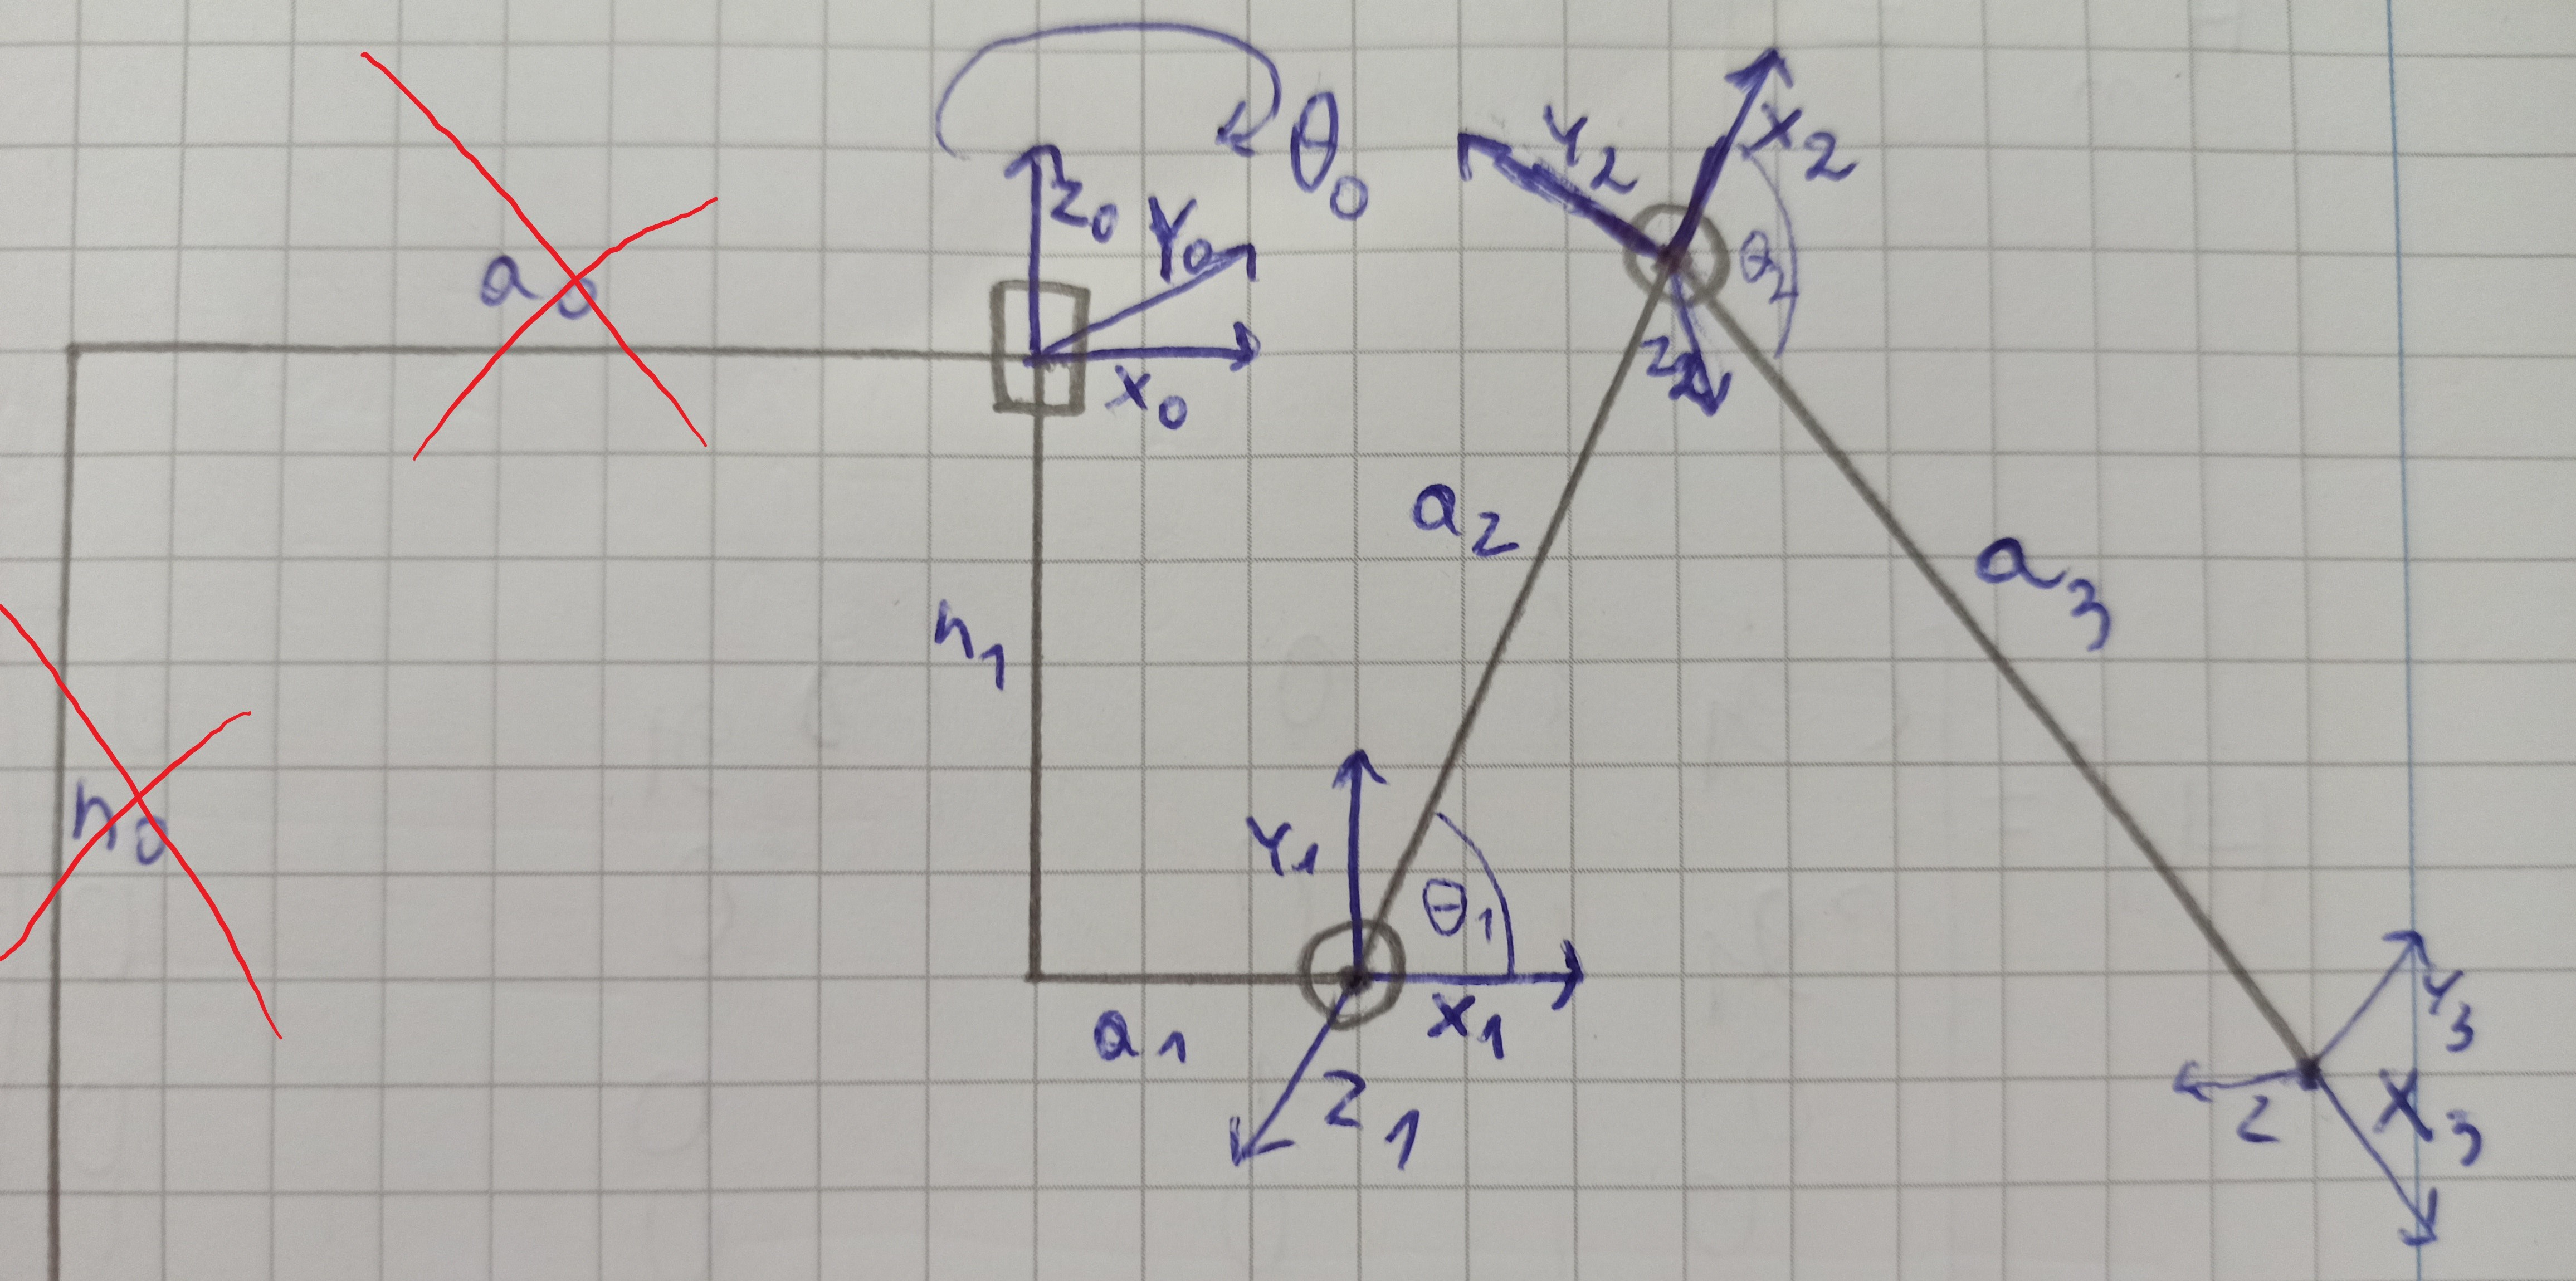
\includegraphics[width=\textwidth]{img/DH_model.jpg}
\caption{Model Denavit Hartenberg}
\label{math_model_DH}
\end{figure}

Z praktycznynego punktu widzenia obliczenia należy zacząć od stworzenia specjalnego rysunku (Rys. \ref{math_model_DH}) z zaznaczonymi kolejnymi obrotami lokalnych układów współrzędnych, a następnie zebrać odpowiednie transformacje do tabelki (Tab. \ref{table:DH_table})\\

\begin{table}[h!]
\centering
\begin{tabular}{c | c c c c }
 Joint $i$ & $\theta_i$ & $\alpha_i$ & $r_i$ & $d_i$ \\
 \hline
 $1$  & $\theta_0$ & $\frac{\pi}{2}$ & $a_1$ & $h_1$ \\
 $2$  & $\theta_1$ & $0$ & $a_2$ & $0$ \\
 $3$  & $\theta_2$ & $0$ & $a_3$ & $0$ \\
\end{tabular}
\caption{Tabela z parametrami DH}
\label{table:DH_table}
\end{table}

Gdzie: \\
$\theta_i$ - angle from $x_{n-1}$ to $x_n$ around $z_{n-1}$\\
$\alpha_i$ - angle from $z_{n-1}$ to $z_n$ around $x_n$\\
$r_i$ - distance between the origin of the $n-1$ frame and the origin of the $n$ frame along the $x_n$ direction.\\ 
$d_i$ - distance from $x_{n-1}$ to $x_n$ along the $z_{n-1}$ direction\\

Następnie macierze transformacji jednorodnej (pomiędzy ramkami $n-1$ i $n$) oblicza się zgodnie ze wzorem \ref{DH_homogenous}. Wzór ten jest właśnie obliczony poprzez wymnożenie wzorów na wyżej wspomniane 6 przekształceń prostych. Ale w zasadzie wzór ten sprowadza się do 2 zasadniczych elementów. $R$ jest macierzą Rotacji o rozmiarze $3x3$ a $T$ to macierz Transformacji $1x3$. \\

\begin{equation} \label{DH_homogenous}
H^{n-1}_n = 
\left[\begin{array}{ccc|c}
&&&\\
&&&\\
\multicolumn{3}{c|}{\smash{\raisebox{0.75\normalbaselineskip}{R}}} & \smash{\raisebox{0.75\normalbaselineskip}{T}}\\
\hline
0 & 0 & 0 & 1\\
\end{array}\right] = 
\left[\begin{matrix}
\cos{\theta_i} & -\sin{\theta_i} \cdot \cos{\alpha_i} & \sin{\theta_i} \cdot \sin{\alpha_i} & a_i \cdot \cos{\theta_i}\\
\sin{\theta_i} & \cos{\theta_i} \cdot \cos{\alpha_i} & -\cos{\theta_i} \cdot \sin{\alpha_i} & a_i \cdot \sin{\theta_i}\\
0 & \sin{\alpha_i} & \cos{\alpha_i} & d_i\\
0 & 0 & 0 & 1\\
\end{matrix}\right]\cite{DH_matrix_AA_article}
\end{equation}


Następnie należy podstawić wartości dla każdego z 3 punktów i otrzymane macierze wymnożyć zgodnie ze wzorem \ref{DH_final_equation}.

\begin{multline} \label{DH_final_equation}
H^{n-1}_n = H^0_1 \cdot H^1_2 \cdot H^2_3 =\\
\left[\begin{matrix}
c\theta_0 \cdot \left( c\theta_1 \cdot c\theta_2 - s\theta_1 \cdot s\theta_2 \right) & -c\theta_0 \cdot \left( c\theta_1 \cdot s\theta_2 + s\theta_1 \cdot c\theta_2 \right) & s\theta_0 & c\theta_0 \cdot \left( a_1 + a_2 \cdot c\theta_1 + a_3  \cdot \left( c\theta_1 \cdot c\theta_2 - s\theta_1 \cdot s\theta_2 \right) \right)\\
s\theta_0 \cdot \left( c\theta_1 \cdot c\theta_2 - s\theta_1 \cdot s\theta_2 \right) & -s\theta_0 \cdot \left( c\theta_1 \cdot s\theta_2 + s\theta_1 \cdot c\theta_2 \right) & -c\theta_0 & s\theta_0 \cdot \left( a_1 + a_2 \cdot c\theta_1 + a_3  \cdot \left( c\theta_1 \cdot c\theta_2 - s\theta_1 \cdot s\theta_2 \right) \right)\\
c\theta_1 \cdot s\theta_2 + s\theta_1 \cdot c\theta_2 & c\theta_1 \cdot c\theta_2 - s\theta_1 \cdot s\theta_2 & 0 & h_1 + a_2 \cdot s\theta_1 + a_3 \cdot \left( c\theta_1 \cdot s\theta_2 + s\theta_1 \cdot c\theta_2 \right)\\
0 & 0 & 0 & 1\\
\end{matrix}\right] = \\
\left[\begin{matrix}
c\theta_0 \cdot c\left( \theta_1 + \theta_2 \right) & -c\theta_0 \cdot s\left( \theta_1 + \theta_2 \right) & s\theta_0 & c\theta_0 \cdot \left( a_1 + a_2 \cdot c\theta_1 + a_3  \cdot c\left( \theta_1 + \theta_2 \right) \right)\\
s\theta_0 \cdot c\left( \theta_1 + \theta_2 \right) & -s\theta_0 \cdot s\left( \theta_1 + \theta_2 \right) & -c\theta_0 & s\theta_0 \cdot \left( a_1 + a_2 \cdot c\theta_1 + a_3  \cdot c\left( \theta_1 + \theta_2 \right) \right)\\
c\theta_1 \cdot s\theta_2 + s\theta_1 \cdot c\theta_2 & c\left( \theta_1 + \theta_2 \right) & 0 & h_1 + a_2 \cdot s\theta_1 + a_3 \cdot s\left( \theta_1 + \theta_2 \right)\\
0 & 0 & 0 & 1\\
\end{matrix}\right]
\end{multline}

Następnie, aby otrzymać właściwe równania, należy z równania \ref{DH_final_equation} wziąć część odpowiedzialną za transformację. Efektem jest wzór \ref{FK_ver_2}, czyli finalna wersja równań kinametayki prostej obliczonej metodą Denavita Hartenberga\\

\begin{equation} \label{FK_ver_2}
\begin{split}
X &= c\theta_0 \cdot \left( a_1 + a_2 \cdot c\theta_1 + a_3  \cdot c\left( \theta_1 + \theta_2 \right) \right)\\
Y &= s\theta_0 \cdot \left( a_1 + a_2 \cdot c\theta_1 + a_3  \cdot c\left( \theta_1 + \theta_2 \right) \right)\\
Z &= h_1 + a_2 \cdot s\theta_1 + a_3 \cdot s\left( \theta_1 + \theta_2 \right)\\
\end{split}
\end{equation}

TODO - znak się nie zgadza


\subsubsection{Invert kinematics}
Kinematyka odwrotna to TODOTODOTODO

Zwykle odwrotną kinematykę można obliczyć poprzez rozwiązanie równań kinematyki prostej. Jest to w tym przypadku także teoretycznie możliwe, jako że mamy do czynienia z trzema niewiadomymi ($\theta_{0-2}$) i układem trzech równań nr. \ref{FK_ver_1} lub \ref{FK_ver_2}. (Równanie na $a_{temp}$ jest jedynie pomocnicze, trzeba je traktować jak część równań $Y$ i $X$).

Jest to jak najbardziej wykonalne w przypadku $\theta_0$, można to zrobić łącząc wzór na $X$ i $Y$, dzieląc go obustronnie, zamieniając $\frac{\sin}{\cos}$ na $\tan$ i wyciągając $\theta_0$ na lewą stronę. Daje to wzór \ref{theta_0_eq_final}

%\begin{equation}
%\begin{split}
%\begin{cases}
%Y = a_{temp} \cdot \sin{\theta_0}\\
%X = a_{temp} \cdot \cos{\theta_0}
%\end{cases}
%\end{split}
%\end{equation}

%\begin{equation}
%\begin{split}
%\begin{cases}
%Y = a_{temp} \cdot \sin{\theta_0}\\
%a_{temp} = \frac{X}{\cos{\theta_0}}
%\end{cases}
%\end{split}
%\end{equation}


%\begin{equation}
%Y = \frac{X}{\cos{\theta_0}} \cdot \sin{\theta_0}\\
%\end{equation}

\begin{equation} \label{theta_0_eq_final}
\theta_0 = \arctan{\frac{Y}{X}}
\end{equation}

%Wzór na $\theta_2$ można wyprowadzić także z równania \ref{FK_ver_1}

%\[
%Z = (- h_1) + a_2 \cdot \sin{\theta_1} - a_3 \sin{\left( \theta_2 - \theta_1 %\right)}
%\]

%\[
%z + h_1 = a_2 \cdot \sin{\theta_1} - a_3 \sin{\left( \theta_2 - \theta_1 \right)}
%\]

%\[
%\frac{h_1 - Z - a_2 \cdot \sin{\theta_1}}{a_3} = \sin{\left( \theta_2 - \theta_1 \right)}
%\]


%\begin{equation} \label{theta_2_eq}
%\theta_2 = \arcsin{\left(\frac{h_1 - Z - a_2 \cdot \sin{\theta_1}}{a_3}\right)} + \theta_1
%\end{equation}

%Równanie \ref{theta_2_eq} jest nadal uzależnione od $\theta_1$, które należy wyznaczyć.

%Najbardziej oczywistym wydaje się pod równanie \ref{FK_ver_1} na $a_{temp}$ podstawić obliczone równanie \ref{theta_2_eq} i daje to równanie  \ref{theta_1_eq1}

%\begin{equation} \label{theta_1_eq1}
%a_{temp} = a_2 \cos{\theta_1} + a_3 \cos{\left(\arcsin{\left(\frac{h_1 - Z - a_2 \cdot \sin{\theta_1}}{a_3}\right)}\right)} + a_1\\
%\end{equation}

%Do fragmentu $a_3 \cos{\left(\arcsin{\left(\frac{h_1 - Z - a_2 \cdot \sin{\theta_1}}{a_3}\right)}\right)}$ można zastosować wzór $\cos{\left(\arcsin{\left(x\right)}\right)} = \sqrt{1 - x^2}$. Daje to wzór \ref{theta_1_eq2}

%\begin{equation} \label{theta_1_eq2}
%a_{temp} = a_2 \cos{\theta_1} + \sqrt{a_3^2 - (a_2 \sin{\theta_1} - h_1 - Z)^2} + a_1\\
%\end{equation}

%Niestety wzór \ref{theta_1_eq2} nie pozwala jednoznacznie wyznaczyć jawnego $\theta_1$ i co za tym idzie nie da się tego wzoru jednoznacznie zaimplementować softwareowo, co jest niezbędne w dalszej części pracy. Można natomiast powrócić do rysunku \ref{math_model} i zastosować na trójkącie utworzonym z $a_2$ i $a_3$ twierdzenie cosinusów połączone z twierdzeniem pitagorasa.

Większy problem pojawia się jednak w przypadku obliczania $\theta_1$ i $\theta_2$, ponieważ wartości te da się obliczyć z wyżej wspomnianego równania, ale nie da się wyznaczyć na te wartości równań w postaci jawnej. A bez postaci jawnej poprawna implementacja tych równań będzie znacznie utrudniona.

Można natomiast zastosować pewnego rodzaju uproszczenie. Jeżeli wyznaczanie równań $\theta_1$ i $\theta_2$ sprowadzi się do problemu dwuwymiarowego, obliczenia stają się w zasadzie identyczne jak w przypadku obliczeń kinematyki odwrotnej dla robota typu SCARA, co było już robione wielokrotnie.\\

Aby obliczyć kąt $\theta_2$ można powrócić do rysunku \ref{math_model} i zastosować na trójkącie utworzonym z $a_2$ i $a_3$ twierdzenie cosinusów połączone z twierdzeniem pitagorasa. Daje to wzór \ref{theta_2_eq_1}.

\begin{equation} \label{theta_2_eq_1}
(x - a_1)^2 + (z + h_1)^2 = a_2^2 + a_3^2 - 2 \cdot a_2 \cdot a_3 \cdot \cos{(180^o - \theta_2)}\\
\end{equation}

Następnie na podstawie równania \ref{theta_2_eq_1} aby ostatecznie otrzymać $\theta_2$ należy zastosować wzór $\cos{(180^o - \theta)} = -\cos{\theta}$ i za pomocą prostych przekształceń wyciągnąć z równania $\theta_2$. Daje to wzór \ref{theta_2_eq_final}

\begin{equation} \label{theta_2_eq_final}
\theta_2 = \arccos{\left( \frac{(x - a_1)^2 + (z + h_1)^2 - a_2^2 - a_3^2}{2 a_2 a_3} \right)}\\ \cite{SCARA_model}
\end{equation}
Natomiast obliczenia dla $\theta_1$ TODO

\begin{equation}\label{theta_1_eq_final}
\theta_1 = \arctan{\frac{z + h_1}{x - a_1}} + \arcsin{\left( \frac{a_3 \sin{\theta_2} }{ \sqrt{ (x - a_1)^2 + (z + h_1)^2}} \right)}\\ \cite{SCARA_model}
\end{equation}

Ostatecznie zbierając równania \ref{theta_0_eq_final}, \ref{theta_1_eq_final}, \ref{theta_2_eq_final} otrzymujemy układ równań który stanowi kinematykę odwrotną opisywanej nogi robotycznej.

TODO - układ równań

TODO - ograniczenia.

Natomiast trzeba cały czas pamiętać że jest to tylko uproszczenie, które będzie owocować pewnymi drobnymi błędami. Trzeba zauważyć, że zmiana współrzędnej $Y$ nie wpływa na wartości kątów $\theta_1$ i $\theta_2$, tylko na $\theta_0$. Oznacza to, że wraz ze zmianą kąta $\theta_0$, na potrzeby uproszczenia obliczeń, obraca się także o ten kąt oś $X$ układu współrzędnych. W praktyce oznacza to, że odsunięcie nogi od punktu $(0, 0, 0)$ zawsze będzie rzutowane na cylinder o promieniu równym odsunięciu o takim samym $X$ i $Z$, ale $Y = 0$. Problem jest zaprezentowany na rysunku XXX. Jednakże błąd powinien być pomijalnie mały a równania powinny umożliwić skuteczną implementację algorytmu chodu.

\subsection{Cały Robot}
Zwykle konstruując roboty wzorujemy się na zwierzętach występujących w naturze. W tym przypadku nie mamy jednak tego luksusu, dlatego na początek należy przyjąć jakieś najbardziej intuicyjne założenie. Dlatego też uznałem że najlepszym rozwiązaniem będzie rozmieścić nogi na jednej płaszczyźnie w równych odstępach - co $120\deg$.

W poprzednim podrozdziale przyjąłem osie układu relatywne do ułożenia początkowego nogi robota. Oznacza to że robot trójnożny będzie miał 3 niezależne osie $x$ i 3 niezależne osie $y$, tylko oś $z$ zgadza się między kolejnymi nogami. Idzie za tym konieczność stworzenia pewnej metody "obracania" wszystkich tych osi $x$ i $y$ do jednego zunifikowanego układu współrzędnych. Pozwoli to obliczyć kinematykę całego robota.

\subsubsection{Matematyka kroku}
Aby móc w prosty sposób napisać później algorytmy chodu i móc się skupić na kolejności przestawiania nóg przez robota, długości i wysokości kroku i innych tego typu aspektach, należy teraz dobrze ten krok sparametryzować. Na podstawie moich poprzednich doświadczeń z podobnymi projektami, uważam że najbardziej intuicyjne będzie sparametryzowanie kroku do:
\begin{itemize}
\item wartości kąta pomiędzy kierunkiem "do przodu" kroku a osią $x$ danej nogi
\item długości kroku
\item wysokości kroku
\end{itemize}



\section{Model CAD i druk 3D}
\begin{figure}[H]
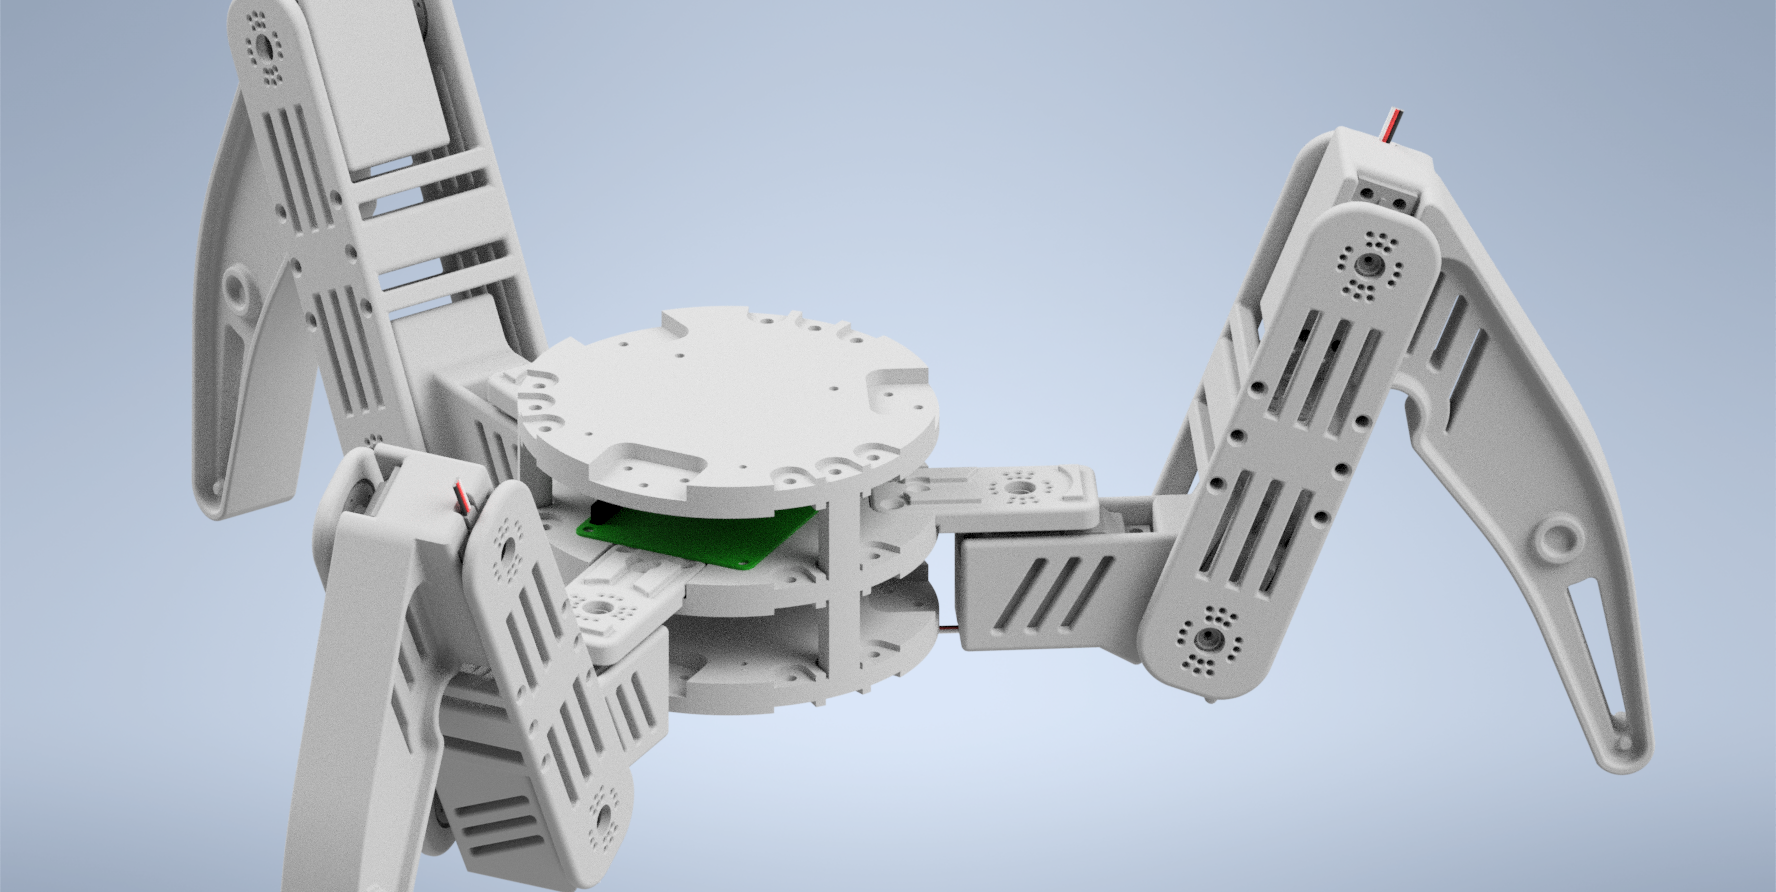
\includegraphics[width=\textwidth]{img/CAD_assembly.png}
\caption{Model Złożeniowy}
\label{CAD_assembly}
\end{figure}
Jedym z głównych założeń projektu była możliwość wydrukowania całej konstrukcji w 3D. Miało to na celu znaczne obniżenie kosztów produkcji, ale przede wszystkim umożliwić znacznie szybsze przeróbki. Jest to o tyle istotne, że prowadzone będą badania z algorytami chodu - przypdaku większości algorytmów wydłużenie pewnych elementów nogi może zmniejszyć wymagane prędkości ruchu serw. Eksperymenty takie mogą wymusić liczne przedruki poszczególnych członów nóg robota.\\

Drugim założeniem projektowym stojącym za konstrukcją taką jak na rysunku \ref{CAD_assembly} jest modularność. Bardzo podobną modularność oferuje robot TurtleBot 3, który także był inspiracją stojącą za konstrukcją. Zarówno Turtlebot jak i konstrukcja budowana w ramach tej pracy składają się z wielu identycznych warstw, które zawierają liczne otwory montażowe umożliwiające przykręcenie w zasadzie dowolnego elemnentu.\\

Zostały także dokładnie zwymiarowane otwory montażowe znajdujące się na orczykach do zakupionych serw i przeniesione na poszczególne elementy nóg. Do montażu wspomnianych orczyków zakupione zostały śruby $M1.6$, co stanowi swojego rodzaju drobny eksperyment. Zwykle orczyki montuje się za pomocą kleju lub wkrętów dostarczanych wraz z serwomechanizmem. Są to jednak metody przynajmniej częściowo destrukcyjne - nie umożliwiają szybkiego demontażu i wymiany elementów, co jest bardzo ważnym elementem tego projektu. Zastosowanie śrub z nakrętkami rozwiązuje ten problem - jednak pojawia się pytanie czy nie generuje to innych problemów? (TODO - tutaj opisać problemy i później we wnioskach odpowiedź czy generuje czy nie czy od razu tutaj polecieć że było git?)\\

Oryginalny projekt zawiera także pewną wadę konstrukcyjną - jest to bardzo cienki element łączący nogę z tułowiem (element nogi zero). Istnieje duże ryzyko gięcia a może nawet łamania się wyżej wymienionego elementu. Aby zmniejszyć to ryzyko, wspomniany element został miejscami pogrubiony i zakupione zostały (TODO - trzeba kupić) metalowe orczyki. Najtrwalszym rozwiązaniem oczywiście byłoby stowrzenie dodatkowego elementu który byłby przytwierdzony do dolnej części obudowy i posiadałby oś obrotu z pierwszym elementem nogi -  "podtrzymywałby" ten elemnt od dołu.\\

Całość konstrukcji została zaprojektowana w programie Autodesk Inventor. Program ten został wybrany tylko i wyłącznie ze względu na fakt, że był autorowi projektu dość dobrze znany. [TODO - opisać problem że szkicy się "rozjeżdżały podczas modyfikowania szkiców "poziomy" niżej czy nie?]\\

Modele zostały wydrukowane na drukarce Zortrax M200. Została ona wybrana ze względu na jej dostępnośc na uczelni. Dodatkowo, aby przygotować pliki pod druk, należało model przetworzyć programem Z-Suite. W programie większość ustawień pozostawiana była bez zmian, jedynie 2 istotne ustawienia zostały dostosowane do projektu. Zostało ustawione minimalne niezerowe wypełnienie, około $10\%$ i warstwy, wierzchnia i spodnia, zostały ustawione na najgrubsą możliwą opcję. Ustawienia te znalezione zostały eksperymentalnie - wydają się najlepiej balansować między wytrzymałością a czasem druku i ilością zużytego materiału. Dodatkowo, przed ostatecznym wydrukiem, wewnątrz programu inventor, zwiększone zostały o około $0.3-0.4 mm$ wszystkie otwory montażowe, ponieważ modele "puchną" i dziury te po wydruku były znacznie mniejsze niż na tworzonych szkicach.\\

\section{Sekcja Elektroniczna}
Projekt elektroniczny na potrzeby tego projektu został ograniczony do minimum. Zasilanie składa się z akumulatora typu LiPo i minimum 2 przetwornic. Jako mózg urządzenia zastosowany został minikomputer Raspberry Pi 4B i to do jego zasilenia potrzebna jest jedna z przetwornic. Zgodnie z dokumentacją Raspberry zasilanie jest ze źródła o napięciu $5V$ i prądzie przynajmniej $3A$.\cite{RPI_power_sup} Dlatego została zainstalowana przetwornica TODO.\\

Druga przetwornica ma za zadanie zasilić serwomechanizmy. Serwomechanizmy wybrane do tego projektu to \href{https://botland.com.pl/serwa-typu-standard/9182-serwo-feetech-ft5715m-standard-5904422312756.html}{Feetech FT5715M} (sztuk 3) i \href{https://botland.com.pl/serwa-typu-standard/3576-serwo-powerhd-lf-20mg-standard-6939670200387.html}{PowerHD LF-20MG} (sztuk 6). W czasie zakupu serwa te wypadały najlepiej spośród wszystkich dostępnych pod kątem prędkości ruchu do ceny. Serwa firmy Feetech są zasilanie napięciem z zakresu $4.8$ do $6V$ a power HD napięciem $4.8$ do $6.6V$. Dlatego jako wspólne napięcie zasilania ustalona została wartość $6V$. Jako że zwykle serwo pobiera do około $1A$ prądu to do ich zasilenia potrzeba przetwornicę o wyjściu $6V$ i minimum $9A$ \cite{Servo_power_sup}. Natomiast należy pamiętać że dobieranie przetwornicy "na styk" przy czymś takim jak zasilanie serwomechanizmów może spowodować później problemy przy większych obciążeniach. Dlatego, aby uwzględnić pewien zapas prądowy, wybrana została przetwornica TODO


\section{Implementacja}
\subsection{Środowisko ROS}
\subsubsection{Schemat implementacji}

\section{Algorytm Chodu}

\begin{thebibliography}{9}

\bibitem{history}
\href{https://www.researchgate.net/publication/258995388_A_Historical_Perspective_of_Legged_Robots}{Manuel F. Silva, J. A. Tenreiro Machado (2006) A Historical Perspective of Legged Robots}

\bibitem{strider}
\href{http://www.romela.org/wp-content/uploads/2015/05/Forward-and-Inverse-Displacement-Analysis-of-a-Novel-Three-Legged-Mobile-Robot-Based-on-the-Kinematics-of-In-Parallel-Manipulators.pdf}{Forward and Inverse Displacement Analysis of a Novel Three Legged Mobile Robot Based on the Kinematics of In Parallel Manipulators}

\bibitem{Triped Martian}
\href{https://www.jstage.jst.go.jp/article/jrobomech/29/3/29_528/_pdf}{Yoichi Masuda, Masato Ishikawa (2017) Simplified Triped Robot for Analysis of Three-Dimensional Gait Generation}

\bibitem{robot_manipulators}
\href{https://books.google.pl/books?id=UzZ3LAYqvRkC&redir_esc=y}{Richard P. Paul (1981) Robot Manipulators: Mathematics, Programming, and Control : the Computer Control of Robot Manipulators}

\bibitem{DH_wpaszke_wyklad}
\href{http://staff.uz.zgora.pl/wpaszke/materialy/air/PRwyklad_4.pdf}{Wojciech Paszke Kinematyka prosta: reprezentacja Denavita-Hartenberga}

\bibitem{DH_AA_article}
\href{https://automaticaddison.com/how-to-find-denavit-hartenberg-parameter-tables/}{How to Find Denavit-Hartenberg Parameter Tables, blogpost by Automatic Addison}

\bibitem{DH_matrix_AA_article}
\href{https://automaticaddison.com/homogeneous-transformation-matrices-using-denavit-hartenberg/}{Homogeneous Transformation Matrices Using Denavit-Hartenberg, blogpost by Automatic Addison}

\bibitem{DH_Matlab_calc}
\href{./DH_calculations.m}{Matlab Denavit Hartenberg calculations}

\bibitem{SCARA_model}
\href{https://sj.umg.edu.pl/sites/default/files/ZN20.pdf}{Adam Labuda, Janusz Pomirski, Andrzej Rak (2009) Model manipulatora o dwóch stopniach swobody}

\bibitem{RPI_power_sup}
\href{https://raspberryexpert.com/raspberry-pi-4-power-requirements/}{Raspberry Pi 4 Power Requirements: Everything You Need to Know}

\bibitem{Servo_power_sup}
\href{https://www.pololu.com/blog/16/electrical-characteristics-of-servos-and-introduction-to-the-servo-control-interface}{Electrical characteristics of servos and introduction to the servo control interface}


\bibitem{}
\href{https://www.diva-portal.org/smash/get/diva2:1462059/FULLTEXT01.pdf}{Alexander Wallen Kiessling, Niclas Maatta (2020) Anthropomorphic Robot Arm}

\end{thebibliography}
\end{document}